%% ------------------------------------------------------------------------- %%
\chapter{Research Methodology}
\label{cap:research}

 \epigraph{
 Work it harder, make it better\\
 Do it faster, makes us stronger\\
 More than ever, hour after hour\\
 Work is never over}
 {Daft Punk}

\paragraphdesc{description of the research: qualitative and quantitative}
This research was conducted following a quantitative and qualitative approach.
The quantitative research evaluated the technologies selected for the experiments, while and the qualitative research gathered data from applications' users.
Data was analyzed and used as basis for improvements of applications based on users expectations.

\paragraphdesc{remember goals: this is where you want to go}
The primary goal of this research, as stated in the first chapter, is to evaluate the current technologies and trends for mobile interaction, whereas 
a secondary goal was to promote the use of mobile technologies by musicians and artists, even without technical knowledge.
These goals seek to bridge the gaps identified in mobile music practices, targeting those who intend to use network technologies and mobile devices for collaborative and cooperative interaction during music performances.


\paragraphdesc{how to define the paths that lead to the goals (this is the methodology!)}
To accomplish these goals, applications were developed to provide working solutions for specific scenarios in mobile music, and experiments were conducted to map possibilities and difficulties found in such scenarios.
The applications developed during this research have their description at Appendix~\ref{ape:applications}, following a chronological order that reflect the research process.
Chapter~\ref{cap:evaluations} presents the network technologies evaluation along with discussions of the use of these technologies and identified constraints.
%%%
\paragraphdesc{evaluate mobile technologies in/for performances}
Technology evaluation follows two patterns. 
Some technologies targeted the automatic exploration of different parameters used in mobile music interaction, different services and routing schemes, and data was gathered over long periods of time.
%; the results and discussion of these evaluations is presented in Chapter~\ref{cap:evaluations}.
%Other technologies were evaluated during actual performances, and are discussed in Chapter~\ref{cap:applications}.
%%
Papers, talks, demonstrations, installations, and performances were the key to accomplish the secondary goal.
The papers, published and presented at several computer music conferences in Brazil and abroad, offered opportunities to reach researchers, musicians, and lay audiences interested in mobile music.
These papers were included in this thesis as Appendix~\ref{ape:papers}

\paragraphdesc{methodologies of past projects from compmus: inspire, cooperate, collaborate}
During the development of this research, other related projects were developed by members of the computer music research group at IME/USP, whose methodologies were considered in this study.
André Bianchi's study of mobile platforms for realtime audio processing~\cite{Bianchi2012ontheperformance} produced the \textit{DSPBenchmarking}, an open source application for Android DSP evaluation.
A partnership with André allowed evaluations of DSP techniques that outperform traditional approaches, with more detail presented in Section~\ref{sec:appdspbenchmarking} from Appendix~\ref{ape:applications}.
Flávio Schiavoni developed an open source tool for network distributed performances with audio and MIDI named \textit{Medusa}~\cite{Schiavoni2011medusa}.
In Flávio's research, network tests using the loopback approach were conducted in order to calculate RTT between desktop computers using different network transport protocols; this methodology was adapted to be used here with mobile devices and different services and routing schemes.


% \paragraphdesc{motivation #1: learn Computer Music}
% \paragraphdesc{motivation #2: learn Mobile Computing}
%%MQZ: motivação é assunto para introdução, aqui me parece meio fora de ordem.


\paragraphdesc{organic research: study, experiment, innovate}
This thesis is also the result of an organic research methodology focusing on alternating periods of studies, experimentation, and innovation.
Periods of studies through courses and books were carried out before the first experiments with each technology addressed, leading to pilot experiments viewed as learning tools.
Issues and alternatives that appeared during these experiments turned out to be valuable resources for periods of brainstorms leading to innovations in the strategies implemented.
To propose innovative solutions and to try them out by developing software were stepstones of the research methodology, that helped identifying gaps and shortcomings which demanded new studies, leading to new research cycles.
%dj: acho que ficou filosófico demais. preciso voltar neste parágrafo novamente.
%%MQZ: veja se ficou mais concreto/claro.

\paragraphdesc{research plan #1: evaluate current options}
The explorative investigation of technologies for mobile music may be categorized in two main branches or research plans.
The first research plan focused on the evaluation of currently explored options from the mobile music state of art, as found in existing literature.
Appendix~\ref{ape:applications} offers a comprehensive description of this first research plan containing the steps dealt with in detail.
% dj: moved to appendix
%Many of the applications developed here are intentionally similar to other applications described in Chapter~\ref{cap:mobilemusic}. 
%At times the idea was to simplify codes and settings for novices, such as in \textit{thereminimal}~(Section~\ref{sec:appthereminimal}) and \textit{pubslides}~(Section~\ref{sec:apppubslides}).
%However, some applications were created to offer solutions for gaps and needs identified in the literature, such as \textit{Sensors2Pd}~(Section~\ref{subsec:appsensors2pd}) and \textit{Sensors2OSC}~(Section~\ref{subsec:appsensors2osc}).
%%%%%
\paragraphdesc{research plan #2: evaluate future (or not) options}
A second research plan is based on exploring options for mobile music from trending mobile technologies that had not been well-known or widespread used in mobile music scenarios. 
These include newer technologies such as IPv6 and gigabit connections, that will be broadly available in the future but aren't yet at the time and place where this research was conducted, and also technologies that were available but didn't yet make their way into mobile music projects, such as Multicast routing and Cloud Services.





%\paragraphdesc{partnership with researchers, musicians, and developers}
%Partnership with musicians, researchers, and developers was a methodological approach for aggregating knowledge and experience from the community of potentially interested parties to this research.
%Many of the performances discussed were only possible due to the musical conception of fellow musicians and artist-researchers.
%Some applications received contributions from the developers' community and also from artist-researchers that collaborated with their development from the initial conception to the evaluation process.
% dj: moved to applications

%\paragraphdesc{create applications for learners}
%\paragraphdesc{create applications for community}

%%MQZ: inverti esses parágrafos, pois os dois últimos parecem menos centrais do que os dois primeiros. Eu tomaria um certo cuidado com a redação pois você não pesquisou softwares para educação musical e também não abordou a literatura de criação coletiva, então seria melhor tratar essas aplicações sociais/educativas como "ensaios exploratórios" para tentar mapear como cloud e mobile poderiam ajudar nessas questões (deixando claro que não são seu foco).

%%dj: retirei os parágrafos, pois realmente não tenho muito mais o que falar, já que seria uma repetição dos goals.

%%%%%%%%%%%%%%%%%%%%%%%%%%%%%%%
\section{Methodology for exploring mobile devices in mobile music}

\paragraphdesc{Android and iOS options}
The focus of this research are mobile devices, especially smartphones.
Exploring mobile devices in real concert situations was the aim of many installations and performances conceived and carried out during this research.
Bearing this in mind, and also the availabity of specific devices within the collaborating research groups, most devices used during application development were Android-based, whereas iOS devices where used in specific partnerships.
Other devices were also used in this research by audiences during web-based collaborative and distributed performances which would only require Internet access. 

%%MQZ: o parágrafo installation and performances havia ficado muito fora de contexto lá no final, trouxe ele pro início e acabei incorporando as frases em outros parágrafos onde tinham mais a ver, ou seja, ele sumiu.
%%\paragraphdesc{installations and performances}

%%
%%\subsection*{Android devices}
%%MQZ: Sem a seção "iOs" (ver comentário correspondente) não faz sentido manter uma seção "Android", o melhor é eliminar essa subdivisão.

\paragraphdesc{open/closed source code evaluation for free: git (open source) or APK (closed source)}
The Android operating system was selected as the main focus for application development during this research for some reasons, one of them being the ease of adopting FLOSS ideals in development.
Applications were developed under free licenses with open sources and became available for use through Github repositories, F-Droid and compiled applications. On one hand, source-based distribution is useful for collaborative development, and on the other hand distribution of compiled versions (apk) is more friendly to interested users and beta testers.
Android also offers possibility of distributing applications through Bluetooth, WiFi, or web pages, without the burden of having to publish them or sign provisioning profiles with a device ID as in the case of iOS applications.

%%%
\paragraphdesc{price of devices}
%Another reason for selecting Android devices in this research was the bare fact that these devices have a larger specification spectrum and are generally cheaper than iOS devices.
%Particularly in Brazil, where most of the research was conducted, Android devices are more popular and have lower prices than iOS devices with similar hardware.

\paragraphdesc{development with Eclipse + ADT}
Android application development was based in two main IDEs.
The Eclipse IDE was used during the development of the first applications, mainly due to its popularity among Android developers.
This IDE requires the Android Development Tools~(ADT) plugin for compiling applications and communicating with Android devices and emulators.
By the end of the research period, the Eclipse ADT became deprecated and the application development moved on to Android Studio.
%%%
\paragraphdesc{development with Android Studio}
Android Studio is the official IDE for the development of Android applications and replaced the Eclipse ADT by the end of 2015~\footnote{An update on Eclipse Android Developer Tools - Android Developers Blog: \url{https://android-developers.googleblog.com/2015/06/an-update-on-eclipse-android-developer.html} (visited on May, 2017)}.
This IDE presents a complete environment offering many tools for debugging and monitoring running applications.
%At the current version it is also possible to update the application code without recompiling the full application, improving application development (as compilation usually takes a long time).

\paragraphdesc{application testing with emulators (why not)}
Emulators allowed running applications together with the IDEs inside the same machine.
This option facilitates interface design and local network simulation.
The emulators used during this research were based on the native images that come with the Android SDK, and also the Genymotion Android Emulator~\footnote{Genymotion Android Emulator website: \url{https://www.genymotion.com/} (visited on May, 2017)}.
Although Android emulators can simulate virtual sensors at their current versions, some applications required the evaluation of sensors and other features unavailable at emulators during the development period and obliged the use of real devices as well.

\paragraphdesc{real devices for testing: devices used during research}
The mobile devices used during this research were LG D686 G Pro Dual Lite, Samsung GT-I9300 Galaxy SIII, and Sony Xperia D8533 (and D8503) Z3 Compact.
Their main technical specifications are presented on the Table \ref{tab:gsmarena-lg-s3-z3-short}, and the complete settings of the devices are described in Appendix~\ref{ape:gsmarena-lg-s3-z3}.
Other personal devices were used during the application development process (by beta testers) and also during the installations (by the audiences), and they were not cataloged.

\begin{longtable}{llp{0.2\linewidth}p{0.2\linewidth}p{0.2\linewidth}}
	\caption{Main technical specifications of the mobile devices used during this research: D686, S3, and Z3. Source: Adapted from \cite{GSMARENA2017-lg-s3-z3}} \\ \hline
	&               & LG D686 G Pro Lite Dual                              & Samsung GT-I9300 Galaxy SIII                                                                  & Sony D8533 (and D8503) Xperia Z3 Compact                                                          \\ \hline \endhead
	LAUNCH   & Announced     & 2013, October                                   & 2012, May                                                                                   & 2014, September                                                                                                \\
	& Status        & Available. Released 2013, November              & Available. Released 2012, May                                                               & Available. Released 2014, September                                                                            \\ \hline
	PLATFORM & OS            & Android OS, v4.1.2 (Jelly Bean)                 & Android OS, v4.0.4 (Ice Cream Sandwich), 4.3 (Jelly Bean)                                   & Android OS, v4.4.4 (KitKat), upgradable to v6.0 (Marshmallow)                                                  \\
	& Chipset       & Mediatek MT6577                                 & Exynos 4412 Quad                                                                            & Qualcomm MSM8974AC Snapdragon 801                                                                              \\
	& CPU           & Dual-core 1.0 GHz Cortex-A9                     & Quad-core 1.4 GHz Cortex-A9                                                                 & Quad-core 2.5 GHz Krait 400                                                                                    \\
	& GPU           & PowerVR SGX531                                  & Mali-400MP4                                                                                 & Adreno 330                                                                                                     \\ \hline
	MEMORY   & Card slot     & microSD, up to 32 GB (dedicated slot)           & microSD, up to 64 GB (dedicated slot)                                                       & microSD, up to 256 GB (dedicated slot)                                                                         \\
	& Internal      & 8 GB, 1 GB RAM                                  & 16/32/64 GB, 1 GB RAM                                                                       & 16 GB, 2 GB RAM                                                                                                \\ \hline
	COMMS    & WLAN          & Wi-Fi 802.11 b/g/n, Wi-Fi Direct, DLNA, hotspot & Wi-Fi 802.11 a/b/g/n, dual-band, Wi-Fi Direct, DLNA, hotspot                                & Wi-Fi 802.11 a/b/g/n/ac, dual-band, Wi-Fi Direct, DLNA, hotspot                                                \\
	& Bluetooth     & v3.0, A2DP                                      & v4.0, A2DP, EDR, aptX                                                                       & v4.0, A2DP, LE, aptX                                                                                           \\ \hline
	FEATURES & Sensors       & Accelerometer, proximity, compass               & Accelerometer, gyro, proximity, compass, barometer                                          & Accelerometer, gyro, proximity, compass, barometer                                                             \\ \hline
	\label{tab:gsmarena-lg-s3-z3-short}
\end{longtable}

\paragraphdesc{iOS}
Some applications for iOS devices using the \textit{\textit{urMus}} platform were developed during the period as an exchange student at the University of Michigan under the supervision of Professor Georg Essl.
Within Professor Essl's group many iOS devices, such as iPods, iPhones, and iPads, were available for research purposes.
A better description regarding this partnership is presented in Section~\ref{sec:partnerships}
%%%%%
\paragraphdesc{\textit{urMus}}
All of these devices had the \textit{urMus} platform installed and this allowed the development of mobile music applications without the need of subscribing to the Apple Developer Program.
A web interface for the \textit{urMus} platform  is available, which allows developers to deploy new codes and interfaces for mobile applications.
The developed applications were tested on real devices and some of them were used during mobile performances by students.
The main evaluation of these applications was made through qualitative reports during demonstrations and rehearsals, and also from feedback by Professor Essl before performances.

\paragraphdesc{web technologies}
Although the development of hybrid solutions has generally been avoided in this research, the creation of applications using web technologies was proposed.
The main web technology considered was Audio Synthesis with Web Audio and network communication through Cloud Services.
The compatibility of the Web Audio API with browsers available for several mobile platforms allows the participation of many users in a mobile music performance without the burden of having to install OS dependent applications, since all interaction and control is done within a web site.


%%%%%%%%%%%%%%%%%%%%%%%%%
\section{Network}

\paragraphdesc{Intranet and Internet alternatives}
Intranet and Internet were used in order to evaluate network alternatives for mobile music interaction and collaboration.
Some network communication options were available only in specific scenarios during the research and the applications evaluated through these solutions aimed to explore most of the available settings.
The comparison of alternative mobile technologies was conducted under similar conditions whenever possible (i.e. when technologies could be employed in similar scenarios).
%%MQZ: essas frases estão bem estranhas, não consigo entender/corrigir:
%%As the research progressed some options were included and others were removed.
%%The main constraints of these technologies were than defined to be evaluated in order to find out some numbers regarding performance on real simulations.

\paragraphdesc{Local network}
Intranet settings evaluations were related to protocols options and other technical aspects.
Most of the evaluations using local networks were made using UDP for packet exchanging between Android devices and through Bonjour for iOS.
An additional evaluation was made using the network infrastructure available for academic institutions, which might be considered an Intranet due to its private access policy and backbone topology.

\paragraphdesc{Academic Networks}
Academic institutions are usually connected through national networks which are in turn connected to other backbone networks in different countries.
The Rede Nacional de Ensino e Pesquisa~(RNP) manages the academic network available for Brazilian universities, while the Internet2 is responsible for interconnecting US universities, and RedCLARA is a network that interconnects Latin America's academic networks.
These interconnected backbone networks were used in this research in order to evaluate long distance communication between Brazil and US.
This academic network allows the use of services available on local networks and also offers public IPs for devices (with the permission of a participating institution).
Due to their private access, the use of these networks was only made possible after registering the research project and participating research groups within the academic network managerial infrastructure.

\paragraphdesc{Internet}
Use of the Internet was an expected approach since this technology is widely accessible.
Although many applications were designed for direct communication, some of them were designed to use Internet technologies such as web services and Cloud Services. These are interesting alternatives which are accessible to lay audiences and non-academic researchers as well.

%%
\subsection*{Web service}
 
\paragraphdesc{web server as first alternative}
A web service was considered as the first option for evaluating the use of solutions for mobile music interaction over the Internet, since
using a web server for web service deployment is a common approach for web developers that want to distribute data between many devices and platforms.
A web server allows the creation of an online application on a shared computer that can be reached by anyone connected to the Internet.

%%Use of a regular desktop computer allows the use of common programming languages and also the simulation on local computers before its use on the web. 
%%Additionally, it is important to know that the performance of a web service depends on the available resources on the web server.

\paragraphdesc{POST and GET approach}
The traditional HTTP requests GET and POST are common options available in APIs developed for web services.
During an interactive performance, the applications are expected to GET the most updated data and POST updated data in order to share with other devices, so the idea of focusing only on these requests was a natural approach for real-time interaction.
Other requests such as UPDATE or DELETE would not be very useful in a real time context where data is immediately used after it is shared, so there is no need to manage previously exchanged data.

\paragraphdesc{Ruby on Rails}
Web service development with an API can be hard for users without technical knowledge.
Bearing this in mind, a Rapid Application Development~(RAD) approach was an interesting alternative for exploration.
The Ruby on Rails~(RoR) framework was selected to create the web application that would run on the web server and offer the required web services for exchanging data between mobile devices.
This framework offers the possibility of creating applications with just a few lines of code, describing the data that will be exchanged and the fields and types of database elements.
This framework is also an alternative for developers who intend to create complete multi-featured web applications without having to create their code from scratch based on a full Model View Controller~(MVC) design pattern.

\paragraphdesc{JSON}
An application created with RoR offers ready-to-use requests for getting, posting, updating, and deleting data, including support for widely-used data formats such as JSON.
This format was used in many applications developed during this research due to its improved readbility and cross-compatibility in comparison to alternatives such as XML.

\paragraphdesc{deploy at Dreamhost shared server + Passenger}
The evaluation of the web service was done in local servers during development, but eventually the application was deployed on a shared web server.
The Dreamhost~\footnote{Dreamhost website: \url{https://www.dreamhost.com/} (visited on May, 2017)} web-hosting plan was used in this case with a shared machine including two 4-cores AMD Opteron(tm) Processors (model 4122) with 32Gb of RAM. 
The Phusion Passenger~\footnote{Phusion Passenger website: \url{https://www.phusionpassenger.com/} (visited on May, 2017)} was the web server and application server installed in this machine in order to offer support for the RoR application.
The setup of these technologies was based on user panels that required little effort in order to get at a complete ready-to-use solution.

%%
\subsection*{Cloud Services}

\paragraphdesc{cloud services as an advantage for musicians and for fast app development/deploy}
%%The idea of using a web server for interactive solutions can be considered a path with many steps, even through the use of RAD and RoR.
Cloud Services were also explored as an alternative to web servers, which offers comparatively less control but faster deployment and also scalability.
This alternative is conceptually similar to a web server solution deployed in a distributed manner, since the Cloud is basically made of many interconnected servers, but this interconnection structure offers some advantages. 

\paragraphdesc{Cloud structure}
Cloud servers offers the possibility of automatic service replication automatically through web interfaces, allowing an application to keep running even if many users decide to access it at the same time.
Although most mobile application experiences on the literature expected the participation of only a few dozens of participants, the audience size can be extended with a scalable technology such as that of a cloud service.
The evaluation of Cloud Services conducted in this research explored setup times, APIs and also the scalability levels of cloud solutions offered by some companies on free and paid plans. 

\paragraphdesc{Pusher and PubNub}
Pusher and PubNub were selected for cloud evaluation due to its popularity.
Both companies offer the possibility of using the cloud infrastructure without any burdens or setup of virtual machines.
The main settings are available through the website of each company, whereas other settings are made available through their APIs.
Although the companies offer demo keys for users aiming to evaluate the services without a commitment, the plans available after the subscription process provide private keys for security data exchanging. 

\paragraphdesc{API available for many languages and systems}
The cloud services APIs used here were designed for Android and Javascript.
The methods were selected to simulate the GET and POST approach defined for web services, to facilitate comparison of both approaches.
In this case, the Cloud Services presented \emph{publish} methods for posting data and \emph{subscribe} methods for getting data.
An important difference between the subscribe approach and the GET request is that, after subscription, all messages are delivered to all users subscribed to the same channel, making this approach lighter than GET. 
Specific keys were used in order to have private channels for communication instead of the demo keys available for user evaluation.

\paragraphdesc{scalability restricted for specific plans: Free, Freemium, or Paid}
The Cloud Service plans selected were the most affordable paid plan and the standard free plan available in both Pusher and PubNub.
These plans had communication limits based on the number of connected devices and the number of exchanged messages per day.
A description of these plans is presented in Table~\ref{tab:pusherpubnubplans}.


%%dj: pegar dados dos serviços na época dos testes -> 2015 ?! ou citar que os valores eram diferentes?!
%%mqz: nem um nem outro, isso não é relevante.
\begin{table}[]
\centering
\caption{Pricing and other details of selected plans from Pusher and PubNub Cloud Services as of 2017. Source:~\cite{Pusher2017website,PubNub2017website}}
\label{tab:pusherpubnubplans}
\begin{tabular}{l|llllll}
Service & Plan         & Price in US\$ & Devices/Day & \multicolumn{3}{c}{Messages} \\ \cline{5-7} 
        &              &               &             & Quantity & Per Second & Size \\ \hline
Pusher  & Sandbox      & Free          & 100         & 200k/Day &    10      & 32kb \\ \cline{2-7} 
        & Startup      & \$49          & 500         & 1M/Day   &    10      & 32kb \\ \hline
PubNub  & Free         & Free          & 100         & 1M/Month & Unlimited  & 32kb \\ \cline{2-7} 
        & Growth Tiers & \$49          & 500         & 2M/Month & Unlimited  & 32kb \\ \hline
\end{tabular}
\end{table}

\paragraphdesc{paid plans used for comparison and performance}
Although the limits of the paid plan and the free plan are similar, these limits are high enough to accommodate traditional mobile music performances as found in the literature. 
The idea of comparing both plans was to figure out whether the paid plan had technical advantages regarding the Cloud technologies.
From the developer point-of-view, the only coding difference between the free or paid plans was the key used to connect to the Cloud Service platform (i.e. there is no significant difference).
The paid plan was used during actual performances to try to avoid problems with limits imposed by the free plan.

\paragraphdesc{Mobile and web applications created}
Some applications were created using Cloud Services that focused on performance and network evaluation.
PubNub was used in the Crowd in C[loud] application described in Section~\ref{sec:appcrowdincloud} from Appendix~\ref{ape:applications}, and this application was evaluated during a real performance described in the same section.
The \textit{PushLoop} application described in Section~\ref{sec:apppushloop} was developed to evaluate both plans and compare their performance with other network alternatives.

\subsection*{Protocols and Routing}

Cloud Services were compared to network alternatives, with several protocols and routing methods.
The protocols used during this research were UDP, IPv4, and IPv6, while the routing methods were Unicast and Multicast.
These options were selected as a baseline reference since they are supposed to be ready-to-use by devices connected to an academic network.

These alternatives offer limits regarding bandwidth throughput and number of connected devices depending on the specific network.
At the University of São Paulo the network managers defined a range of 8 IPs~(a subnet with a CIDR /29) to be used with IPv4 and IPv6 in this research.
This setting allowed 5 devices to be connected at the same time, the other 3 IPs being reserved for gateway, router and broadcast.
At the University of Michigan the devices were registered on the network using their MAC addresses with IPs specified by the network managers.
In both universities devices were connected to the network through specific VLANs that offered public IPs with Intranet and Internet access.

\subsection*{Network constraints evaluated}
%%% network constraints evaluated

During the network evaluation, parameters were defined for simulating specific performance constraints.
The number of packets per second was varied by introducing a delay between packets of up to 1000~ms, and packet sizes varied from 1 to 250 32-bit floating-point values. These parameters were taken to represent typical rates and values that could be acquired from mobile sensors and inputs, either in single events or grouped events.
These values were used for the comparison of the network alternatives described above, as detailed in Chapter~\ref{cap:evaluations}.


%%%%%%%%%%%%%%%%%%
\section{Music Processing}

The mobile music scenarios addressed in this research always considered that audio synthesis and processing took place within mobile devices, and that network communication was mainly used for symbolic and control data. The reasons for this assumption is twofold: on the one hand, previous work at the Computer Music research group at IME/USP~\citep{bianchi2014processamento} already indicated that most Android devices back in 2012 were able to process audio in real-time; on the other hand, not only latency and jitter in network audio transmission were important factors for mobile devices (mostly connected wirelessly), but transmission costs due to mobile data plans also rendered audio streaming less appealing in scenarios with large audiences. Some programming languages specifically designed for music and audio processing were at the core of many applications proposed here.

%%MQZ: não faz sentido ter subseções de um parágrafo ou uma frase.
%%MQZ: muitas frases abaixo não têm a ver com metodologia e estão difíceis de entender, por isso sugeri simplesmente tirá-las.

%%\subsection*{Pure Data}
\paragraphdesc{Pure Data}
Pure Data was the main computer music language used in this research, and is used in the applications described in Sections~\ref{sec:appthereminimal}, \ref{subsec:appsensors2pd}, and \ref{sec:apphoketus} from Appendix~\ref{ape:applications}.
%%The language was also selected to create a course to introduce computer music lessons at the summer courses available at the IME-USP.
%%This course was ministered in 2016 and 2017 and is expected to continue as part of the program in the next years.
%%
%%
%%\subsection*{CSound}
\paragraphdesc{Csound}
The CSound language was used for the development of the application \textit{Touches On The Line}, described in Section~\ref{sec:apptouchesontheline} from Appendix~\ref{ape:applications}.
%%This application development took advantage of the examples available for this language and was used to introduce the concept of collaborative performances through web services.
%%
%%
%%\subsection*{SuperCollider}
\paragraphdesc{SuperCollider}
SuperCollider was used in the development of the collaborative and cooperative live coding application named \textit{SuperCopair}, which is presented in Section~\ref{sec:appsupercopair} from Appendix~\ref{ape:applications}.
%%This language was selected due to its availability on the Atom.io platform which served as the IDE for the live coding performances.
%%The Cloud Services were used in this application and some distributed experiences were then scheduled during this research with members of the SuperCollider discussion list.

%%\subsection*{Web Audio}
\paragraphdesc{Web Audio}
The applications developed for mobile music interaction through a web browser were created using the Web Audio API for audio synthesis.
%Although many libraries have been created for facilitation the use of Web Audio, the audio synthesis was programmed with native Web Audio API functions in all applications.
Section~\ref{sec:appcrowdincloud} and \ref{sec:appbandaaberta} from Appendix~\ref{ape:applications} describe the applications \textit{Crowd in C[loud]} and \textit{Open Band}, respectively, that used Web Audio for music processing.

%%
%%\subsection*{STK}
\paragraphdesc{STK at \textit{urMus}}
During the development of applications for iOS devices the \textit{urMus} platform was used, where audio synthesis is done using the STK.
Music synthesis can be programmed using the flowboxes in the \textit{urMus} interface or with the Lua language flowboxes abstractions.


%%%%%%%%%%%%%%%%%%%%
\section{Partnerships}
\label{sec:partnerships}
Partnerships were established as a way to leverage research and profit from external contributions while at the same time applying in practical situations theoretical work developed for the sake of exploring possibilities in mobile music.
Some partners were selected based on a perceived synergy between their projects and this research, while others appeared after discussions and proposals based on ongoing research. In the following, a few of the interacting research groups and projects which contributed to the methodology adopted are briefly described.
%% Although the partnerships are an odd member of traditional methodologies, this worked relied entirely on them to happen in confidence with the goals.

%%
\subsection*{Computer Music Research Group}
\paragraphdesc{Compmus}
This research was conducted within the Computer Music (CompMus) Research Group at IME-USP, which provided many opportunities for partnerships and exchanging ideas.
Regular weekly discussions allowed the diffusion of particular research problems by group members and also provided a space for research interactions and intersections.

\paragraphdesc{Medusa and Flavio}
A project focused on multichannel audio transmission over computer networks was led by Flávio Luiz Schiavoni and overlapped the beginning of this research.
His project's questions provided many opportunities for discussions regarding the many ways of dealing with data transmission over network protocols.
Many insights and alternatives for music collaboration came from the experiments and performances using the Medusa framework created by Flávio.

\paragraphdesc{André Bianchi and DSPBenchmarking}
A project focused on realtime audio processing in mobile devices and developed by André Jucovsky Bianchi provided many essential interchanges of ideas during the preliminary/defining stages of this research.
Setting up a partnership with Bianchi was a natural move based on my initial interests with Android application development and audio processing evaluation.
The result of this partnership was the contribution in the development of the application \textit{DSPBenchmarking} and of some algorithms evaluated through this tool, and is described in Section~\ref{sec:appdspbenchmarking} from Appendix~\ref{ape:applications}.

\paragraphdesc{Gilmar Dias, Thilo Koch, Guilherme Feulo and technical support}
Many evaluations here presented had to be coordinated between places and groups far away from each other, requiring the recruitment of volunteers to participate in the setups, who besides helping to conduct the evaluations also made contributions to this research.
Gilmar Rocha de Oliveira Dias, Thilo Koch, and Guilherme Feulo do Espírito Santo participated actively during most of the experiments with the \textit{PushLoop} application described in Section~\ref{sec:apppushloop} from Appendix~\ref{ape:applications}.

\paragraphdesc{Fábio Goródscy and Banda aberta with Web Audio}
Another important partnership formed towards the final stages of this research was with Fábio Goródscy, whose research interests started with the exploration of the Web Audio API.
He had developed the \textit{Open Band} project in collaboration with Ariane Stolfi (from the NuSom group discussed below) for audience interaction based on sampling, and we decided to build together a new lightweight version using only the Web Audio API, which is presented in Section~\ref{sec:appbandaaberta} from Appendix~\ref{ape:applications}.


%%
\subsection*{NuSom – Research Center on Sonology}

\paragraphdesc{NuSom}
The Research Center on Sonology~(NuSom) is an interdepartmental research group that congregates the Computer Music Research Group at IME-USP and the Sonology research group at the School of Communication and Arts (ECA-USP), formed by artists-researchers interested in sound studies, composition,  performance and improvisation and their relationships with technology.
\paragraphdesc{Group meetings, Fernando Iazzetta and Rogerio Costa}
The partnership between these groups is strengthened by regular meetings, in which the members discuss text, projects, and performances.

\paragraphdesc{Julian Jaramillo Arango, Vitor Kisil Miskalo and the Network Music}
As this project was beginning to take form, members of NuSom were involved in network music concerts connecting musicians at USP with other centers such as SARC/QUB (Ireland), CCRMA/Stanford (USA) and IRCAM (France).
Even though no partnerships were formed at that time, their work served as motivation for considering distributed performance scenarios, and their approaches and solutions contributed to the development of this research.

\paragraphdesc{André Bandeira and Música Mobilis Crítica}
André Damião Bandeira was a contemporary NuSom composer and researcher studying mobile music and aiming to use some new technologies for his projects and performances.
A collaboration emerged that led us to the development of \textit{Hoketus} presented in Section~\ref{sec:apphoketus} from Appendix~\ref{ape:applications}, which merged many technological and musical concepts into a musical distributed installation.

%%MQZ: tudo isso é repetição do que já apareceu antes...
%\paragraphdesc{Ariane Stolfi and Banda Aberta}
%The project \textit{Open Band} was discussed and even rehearsed many times during NuSom meetings, under the coordination of Fábio Goródscy and Ariane Stolfi.
%Ariane is an architect and her research focus on audio-visual interaction.
%She proposed an initial mobile performance based on many audio samples, however, due to the size of the files, this performance was restricted to local networks.
%The collaboration with this project came with the proposal of adopting a complete audio synthesis using Web Audio and is described at Section~\ref{sec:appbandaaberta}


%%
\subsection*{Residuum}

\paragraphdesc{Sensors2OSC: Thomas Mayer at pure data discussion list}
The Pure Data discussion list is the main place for posting questions and solutions for Pure Data users.
The collaboration with Thomas Mayer from Residuum (https://www.residuum.org/) took place after his post on that list regarding the idea of using Android sensors to control Pure Data patches.
At this time, \textit{Sensors2Pd} was already published and running on the \textit{Hoketus} installation.
This interaction through the list offered us the opportunity to start a collaboration within a larger project named Sensors2, described in Section~\ref{sec:appsensors2} from Appendix~\ref{ape:applications}.

The collaboration with Thomas resulted in the development of \textit{Sensors2OSC} application, an improvement of \textit{Sensors2Pd}, and many other ideas for applications.
This project is receiving contributions from other developers around the world and the current applications are translated in four languages (English, German, Portuguese and Japanese).

%%
\subsection*{University of Michigan}
\paragraphdesc{University of Michigan: Georg Essl, Sang Won Lee, Biqiao Zhang, and Zachary Boulanger}

%%
%\subsection*{Collaborations with the University of Michigan}
%%MQZ: Essa seção não fala praticamente nada iOS, mas sim do período sanduíche. Com esse formato ela não cabe dentro da seção "Methodology for exploring mobile devices in mobile music", e seria melhor movê-la para a seção "Partnerships" (onde está prevista uma seção sobre a UMich).

\paragraphdesc{exchange student at UMich}
A period as an exchange student at the University of Michigan was planned during this research project in order to develop partnerships and also to create opportunities for evaluating long distance communications.
The research group at the University of Michigan headed by Professor Georg Essl was a natural choice due to their experience with mobile music solutions and their research involving applications for mobile platforms such as Android and iOS devices.
Other members of the group were also invaluable partners, such as Sang Won Lee, Qi Yang, and Biqiao (Didi) Zhang.

\paragraphdesc{\textit{urMus}}
An important aspect of the collaboration with professor Essl was the opportunity of working with the \textit{urMus} platform, developed by him.
This platform was designed as a complete mobile solution for mobile music experiences that works both in Android and iOS devices.
The development of applications for \textit{urMus} is made using the Lua language through a web interface, and many of those have been created by students from many different fields, such as computer science, engineering, and arts. The fact that the \textit{urMus} platform can be programmed by students with such diverse backgrounds became a focus of interest for this research. 
%
%%MQZ: melhor não ter esse \paragraphdesc{Lua language}
%%Although \textit{urMus} uses Lua for scripting application interfaces in most of its examples, this language can also be used for programming any kind of application embedded into the \textit{urMus} platform.
%%MQZ: Sem querer apaguei duas frases sobre Lua, minha intenção era apenas comentá-las, pois não tinha nada a ver com o contexto. Também achei a frase anterior bem perdida em relação ao resto, por isso sugeri comentá-la.

\paragraphdesc{deploy new app interface from web}
% The web interface used for programming \textit{urMus} applications is accessible from any browser on both desktop and mobile devices, using IP and port of a specific device running the \textit{urMus} startup (a server).
% This IP can be accessed by devices sharing the same local network if the server has a private IP, or by any device in case of a public IP.
%%dj: essa parte também não combina com parceria ou vantagem de parceria

\paragraphdesc{local network}
A local network at the University of Michigan was used during the whole research with iOS devices.
Application development with the \textit{urMus} platform was mostly based on the knowledge acquired while auditing the multidisciplinary course ``Building a Mobile Phone Ensemble'', taught by Professor Essl in 2015.
In this course, many exploratory exercises were proposed, freeing students' creativity leading to many interesting/unpredictable applications.
The idea of exploring local networks within some exercises was an opportunity to evaluate mobile music interaction strategies in this context, with first attempts related to Unicast, Multicast, and the Bonjour technology.
These experiences are described in Section~\ref{sec:appsumich} from Appendix~\ref{ape:applications}. 

%%
\subsection*{LAViD and RNP}
\paragraphdesc{Carlos Carvalho, LAViD, RNP, Internet2, IRTF, NOCs, PoPs}

Other partnerships occurred during this research that deserve mention.
Long distance communication with mobile devices situated at the Federal University of Paraíba was made possible due to the contact with the student Carlos André Lacerda de Carvalho, member of the Digital Video Applications Lab~(LAViD).
The setup for long-distance communication was made possible with the help of RNP team, especially the system analyst Valter Pereira.


%These partnerships are discussed in Chapter~\ref{cap:evaluations} about evaluations.




%% ------------------------------------------------------------------------- %%
\section{Network evaluation on Android: PushLoop}
\label{sec:apppushloop}

During this research, many network technologies were evaluated through a simple application.
The code of this application was organized to work as an example of how user can communicate through the network options selected and the whole codification was simplified by its maximum.
The main intention was is to provide an easy way to exchange messages between mobile devices around the world with minimum codification effort.
The application created for this evaluation was named PushLoop and included settings for evaluating Unicast IPv4, Unicast IPv6, Multicast, and Cloud Services.

PushLoop Android application is based on the loop-back concept, so one device would send messages, the ``\textit{sender}'', while the other device, the ``\textit{loopback}'', would answer the message as soon as possible, simulating a loop-back circuit.
The first device registered all messages sent and received on a report file with millisecond time-stamp precision.
The method used to register the events on the report was \textit{SystemClock.elapsedRealtime()}.
We also run AsyncTask invoking \textit{executeOnExecutor()} with \textit{THREAD\_POOL\_EXECUTOR} in order to have parallel execution on Android.
The messages had five divisions: a unique device id; message number with cycle number on the range of thousands; the total number of messages; a random integer as a key for message identification; and a block of floats.
An example of a message used during the tests is presented below:

\begin{footnotesize}
	\begin{center}
		23.0.1.A87422113 1001 1000 76 [0.28506452]
	\end{center}
\end{footnotesize}

An activity diagram is presented on Figure~\ref{fig:pushloopactivityDiagram} representing the point of view of a sender activity on the application.
The class diagram is presented on Figure~\ref{fig:pushloopclassdiagram}.
This diagram includes all class from the current version of the application after many changes during the development process due to network experimentation.
Screenshots of the PushLoop application are presented on Figure~\ref{fig:pushloopscreenshots}.

\begin{figure}[!ht]
	\centering
	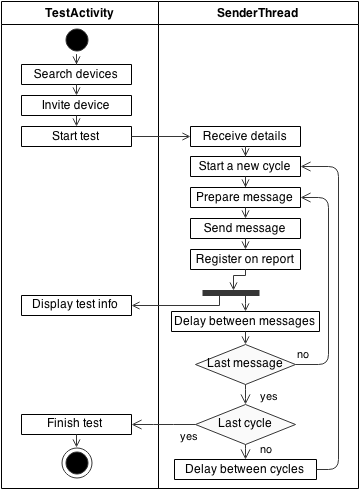
\includegraphics[width=0.40\columnwidth]{testActivityDiagram-BW}
	\caption{PushLoop activity diagram of the test from the sender point of view.}
	\label{fig:pushloopactivityDiagram}
\end{figure}

\begin{figure}[!ht]
	\centering
	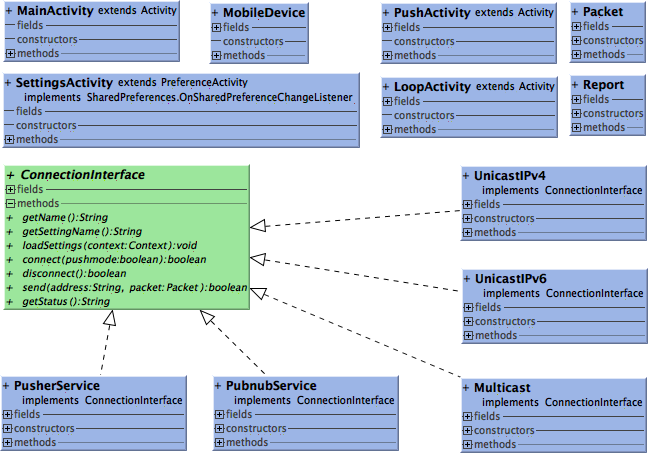
\includegraphics[width=\columnwidth]{PushLoop_ClassDiagram}
	\caption{PushLoop class diagram.}
	\label{fig:pushloopclassdiagram}
\end{figure}

\begin{figure*}[!ht]
	\centering
	\begin{subfigure}{.20\textwidth}
		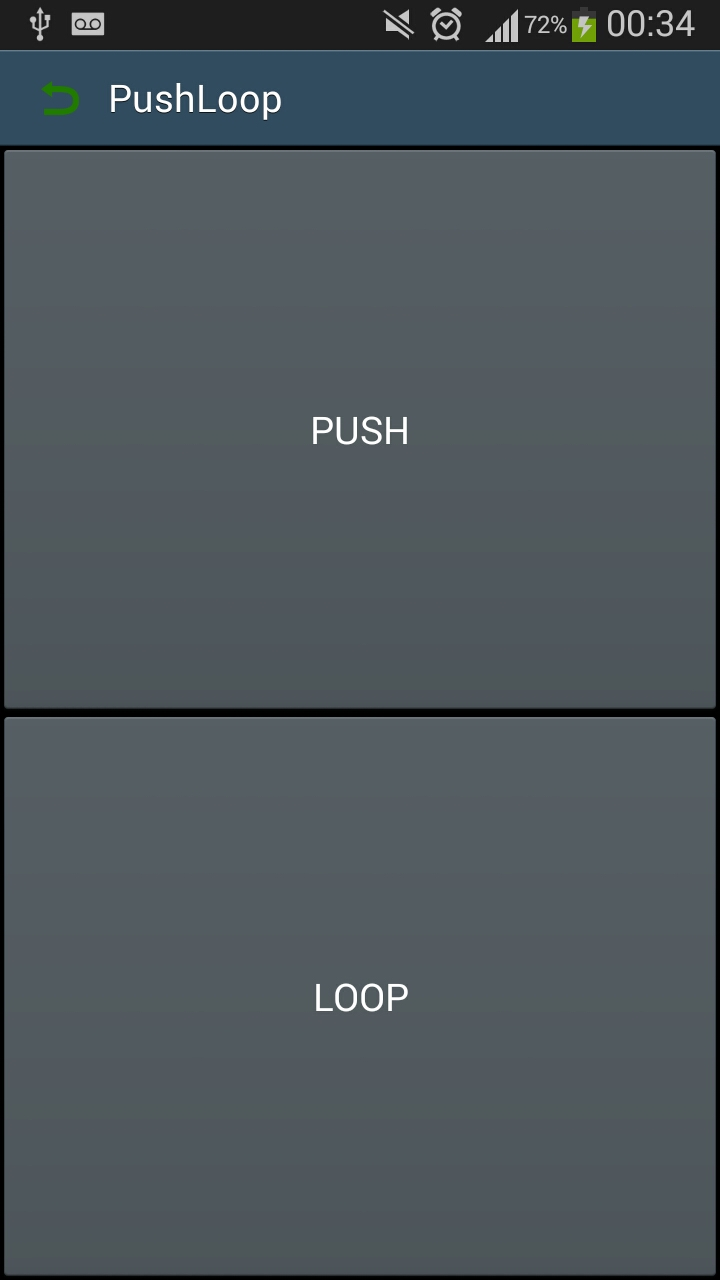
\includegraphics[width=\columnwidth]{pushloop_screenshot}
		\caption{Main screen}
		\label{fig:pushloopss1}
	\end{subfigure}
	\begin{subfigure}{.20\textwidth}
		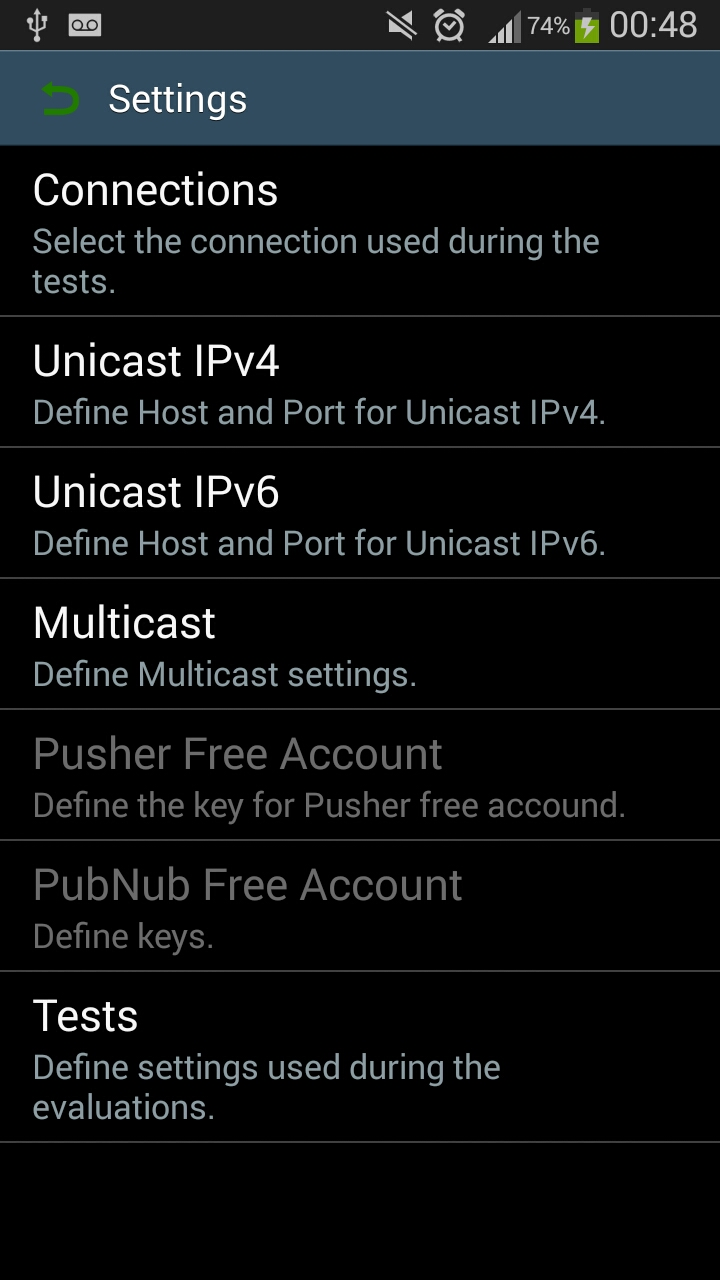
\includegraphics[width=\columnwidth]{pushloop_screenshot2}
		\caption{Settings screen}
		\label{fig:pushloopss2}
	\end{subfigure}
	\begin{subfigure}{.20\textwidth}
		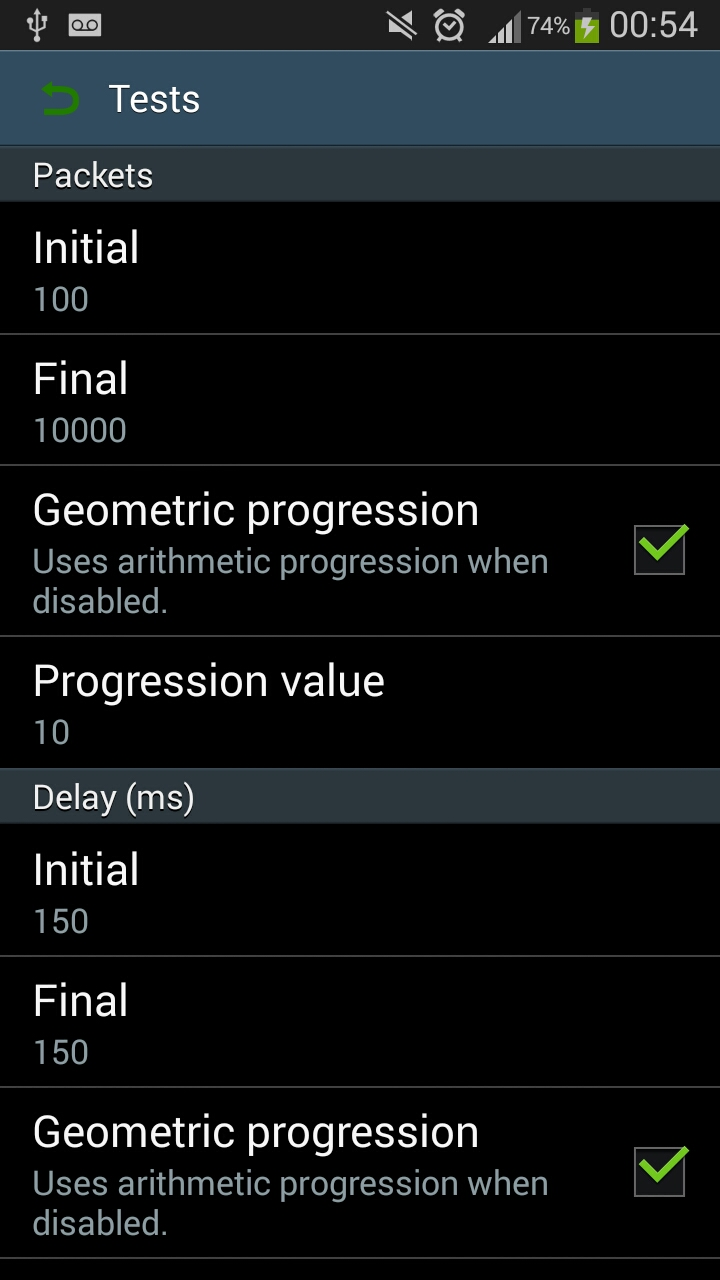
\includegraphics[width=\columnwidth]{pushloop_screenshot3}
		\caption{Test settings screen}
		\label{fig:pushloopss3}
	\end{subfigure}
	\begin{subfigure}{.20\textwidth}
		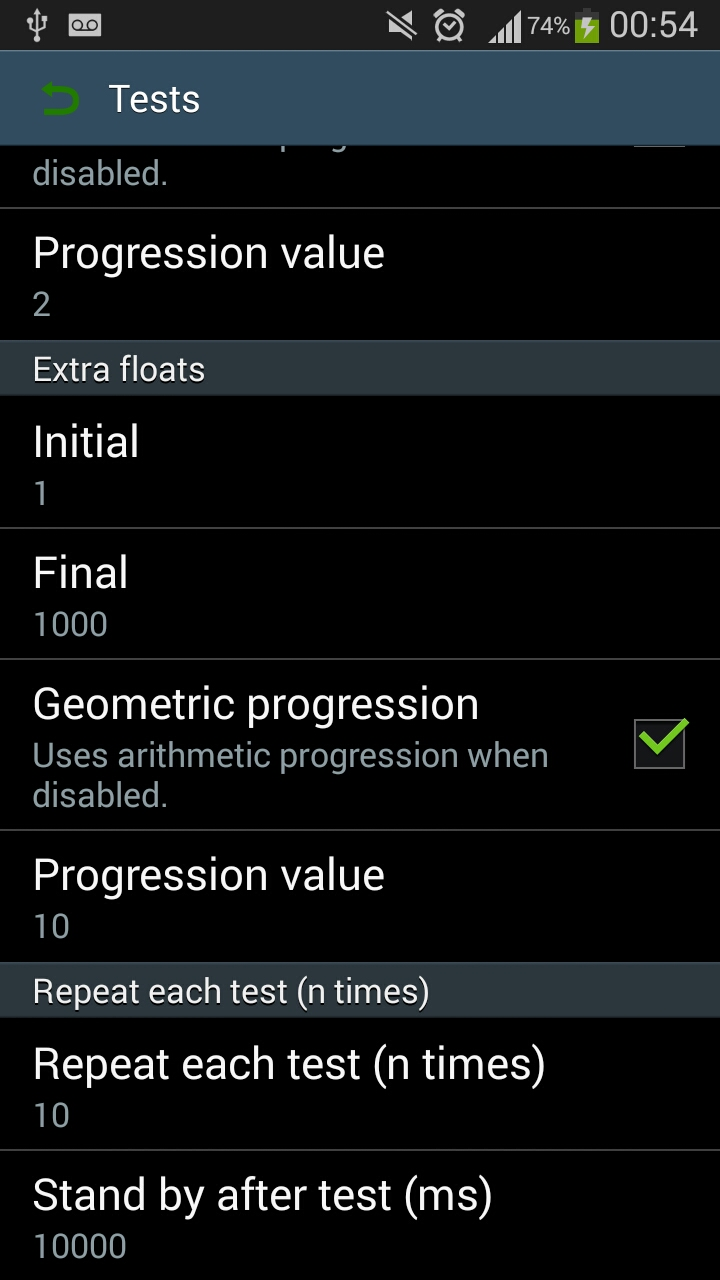
\includegraphics[width=\columnwidth]{pushloop_screenshot4}
		\caption{Test settings screen continuation}
		\label{fig:pushloopss4}
	\end{subfigure}
	
	\caption{PushLoop application screenshots.}
	\label{fig:pushloopscreenshots}
\end{figure*}

The code of the application is available at \url{https://github.com/deusanyjunior/PushLoop} (visited on May, 2017). 
The first evaluation using this application was published as a paper at the International Computer Music Conference, 2015, Denton, Texas, in 2015~\citep{deCarvalhoJunior2015computer}.
This paper is presented at Appendix~\ref{ape:papericmc2015}.
The Chapter~\ref{cap:evaluations} is based on the evaluations conducted with this application.

